\newpage
\section{Mourning Tweets}

El desarrollo y código fuente de esta sección de la tarea se encuentra en el cuaderno \texttt{HW02\_4.ipynb} adjunto.

\subsection{Mourning Lexicon}

\subsubsection{Procesamiento de los \textit{Tweets}}

Antes de realizar la construcción de los \textit{Lexicones} e implementar los modelos de clasificación se realizó un proceso estándar para \textit{tokenizar} los \textit{tweets}. Para esto se hizo un procesamiento especial pensado en lenguaje especifico que se utiliza en \textit{Twitter} y las particularidades de ruido que este medio conlleva. Para esto se realizaron los siguientes pasos:

\begin{itemize}
    \item Remover la puntuación de los \textit{Tweets}.
    
    \item \textit{Tokenizar} el \textit{dataset} con el \textit{tokenizador} (\texttt{TweetTokenizer}) de \texttt{nltk} especializado para este tipo de datos. Esta herramienta:
    \begin{itemize}
        \item Estandariza todas las palabras a minúsculas.
        
        \item Reduce la longitud de las palabras en caso de repetir letras.
        
        \item Remueven caracteres especiales de \textit{Twitter} y usuarios (\textit{@}).
    \end{itemize}
    
    \item Se remueven \textit{stop\_words} utilizando el set de palabras de \texttt{nltk} para cada uno de los idiomas (inglés y español).
    
    \item Con los términos (\textit{tokens}) de los \textit{tweets} se construye un vocabulario (o \textit{dictionary}) para cada uno de los \textit{datasets} (inglés y español). 
    
    \item Con la función \texttt{filter\_extremes} de \texttt{Gensim} se remueven los términos (\textit{tokens}) menos comunes, aquellos que aparecen en menos de 5 documentos (\textit{tweets}). También se hace lo mismo para los más comunes, aquellos que aparecen en más del 75\% del \textit{dataset}, pero este cambio no tuvo efecto en el tamaño del diccionario (posiblemente porque al remover las \textit{stop\_words}, se eliminan las polabras más comunes del \textit{dataset}).
    
\end{itemize}

\subsubsection{Construcción de lexicones}

Una vez se tienen definido el diccionario para los dos datasets, se construyen los lexicones estimando la probabilidad de que cada uno de los términos (\textit{tokens}) este en cada clase (luto o no luto). En este caso, la clase \textbf{luto \textit{(mourning)} se modela como la clase positiva} ($c = 1$) y la clase de \textbf{no luto \textit{(no mourning)} se modela como la clase negativa} ($c = 0$). \\

Para estimar dichas probabilidades, se utilizan los conceptos de verosimilitud  (\textit{likelihood}) y de verosimilitud escalada (\textit{scaled likelihood}). Las expresiones para dichas probabilidades son adaptadas de la referencia \cite{Potts2010SALT}, y se presentan a continuación:

\begin{equation}
    P(w|c=i) = \frac{f(w,c=i)}{\sum_{w\in C} f(w,c=i)}
    \label{likelihood}
\end{equation} \\

Al escalar esta probabilidadc condicional con las probabilidades \textit{a priori} de las palabras y las clases (utilizando el teorema de Bayes), se obtiene la siguiente probabilidad condicional:

\begin{equation}
    P(c=i|w) = \frac{P(w|c=i) p(c=i)}{p(w)} = \frac{P(w|c=i)}{\sum_{c\in C} P(w|c=i)}
    \label{scaled_likelihood}
\end{equation} \\

En \cite{Potts2010SALT}, sugieren trabajar con esta segunda probabilidad condicional pues un sentido más acorde. Dada la palabra, cual es la probabilidad que pertenezca a la clase. No obstante, para los dataset en cuestión se analizan ambas probabilidades.

\subsubsection{Resultados}

A partir de las expresiones (\ref{likelihood}) y (\ref{scaled_likelihood}), se calculan las probabilidades de cada termino para la clase mourning ($c=1$) en los dos datasets (inglés y español).

\begin{table}[H]
    \centering
    \caption{Resultado de los 15 términos con mayor probabilidad de aparecer en tweets de luto (\textit{mourning}) del \textit{dataset} en español (ES).}
    \label{tab:es_lexicons}
    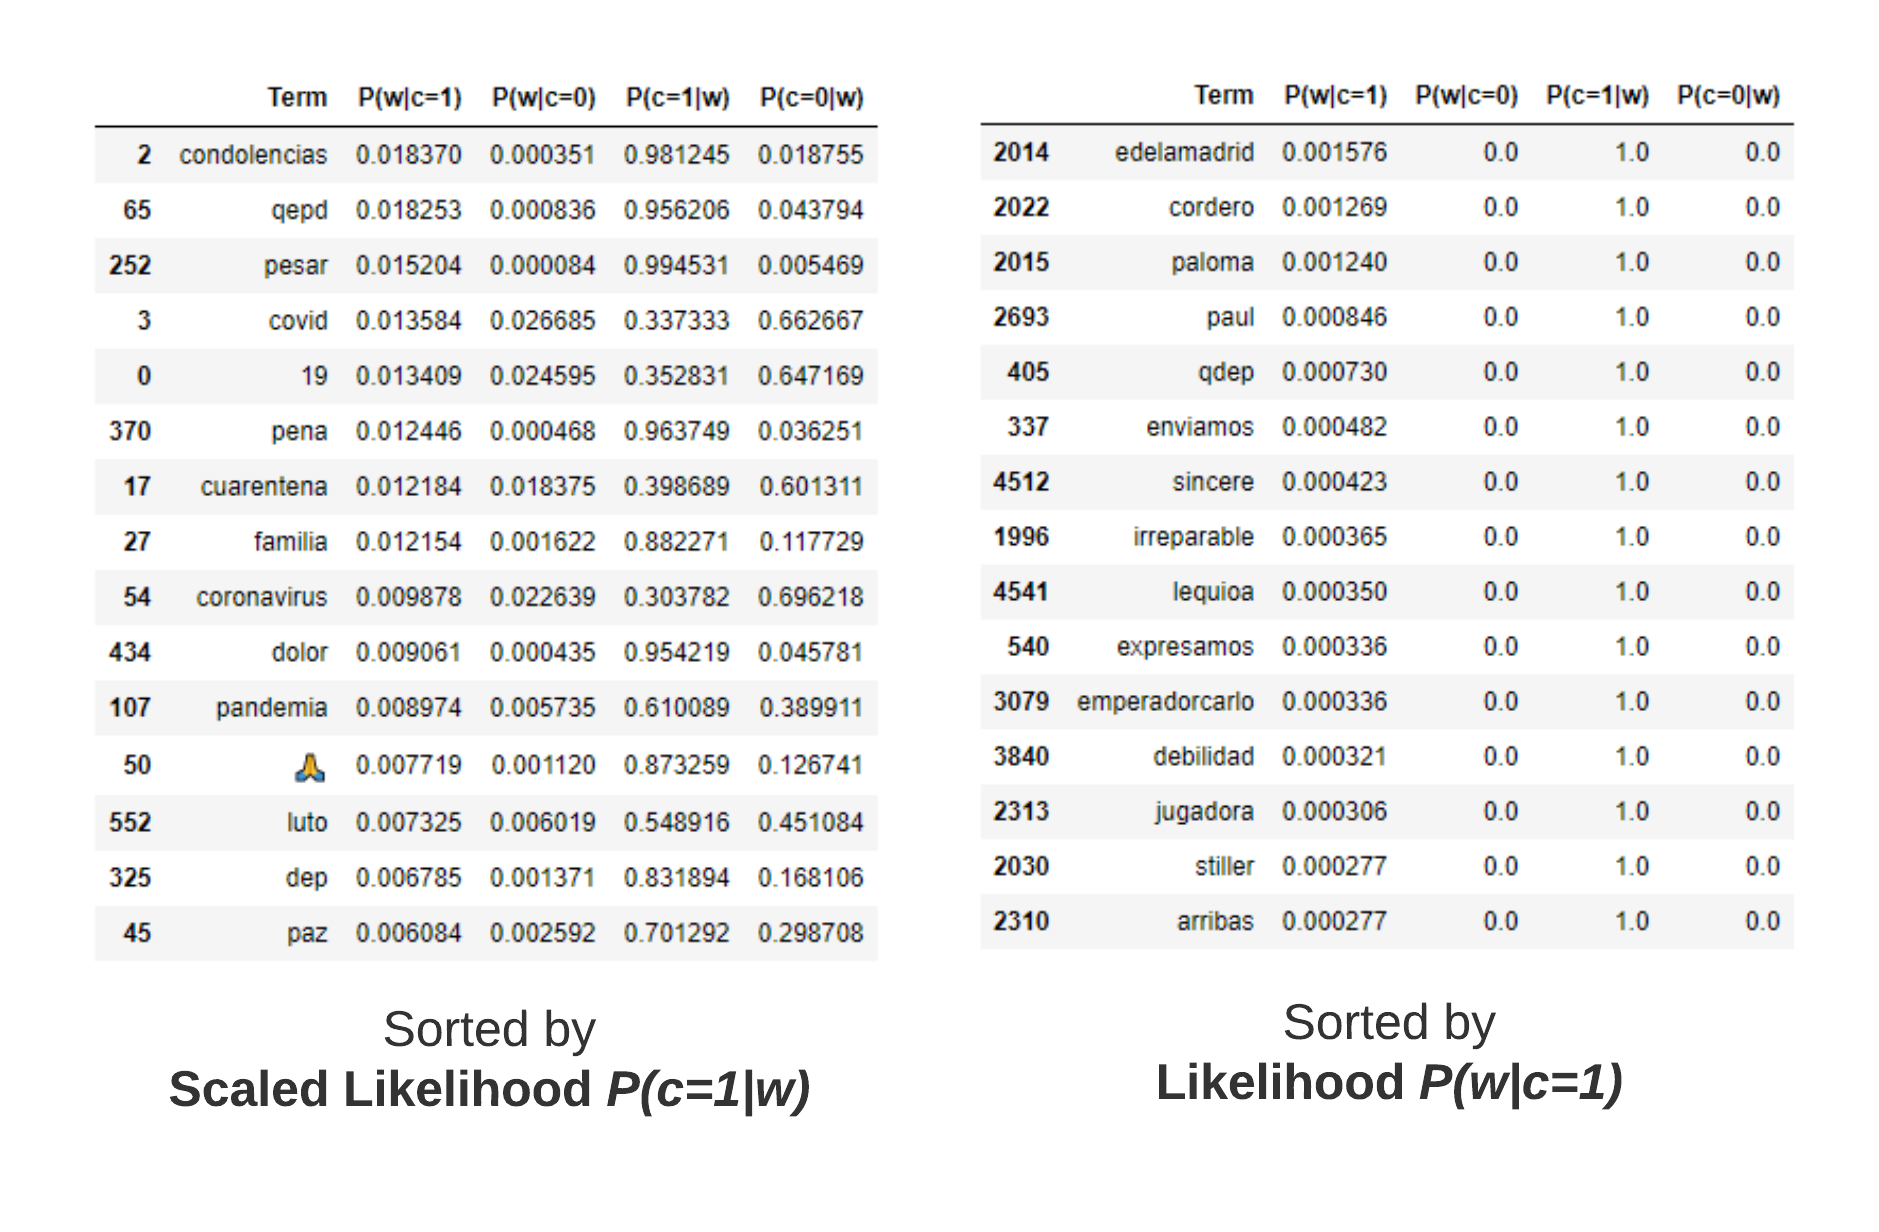
\includegraphics[width=\textwidth]{doc/images/ES_Lexicons.png}
\end{table}

\begin{table}[H]
    \centering
    \caption{Resultado de los 15 términos con mayor probabilidad de aparecer en tweets de luto (\textit{mourning}) del \textit{dataset} en inglés (EN).}
    \label{tab:en_lexicons}
    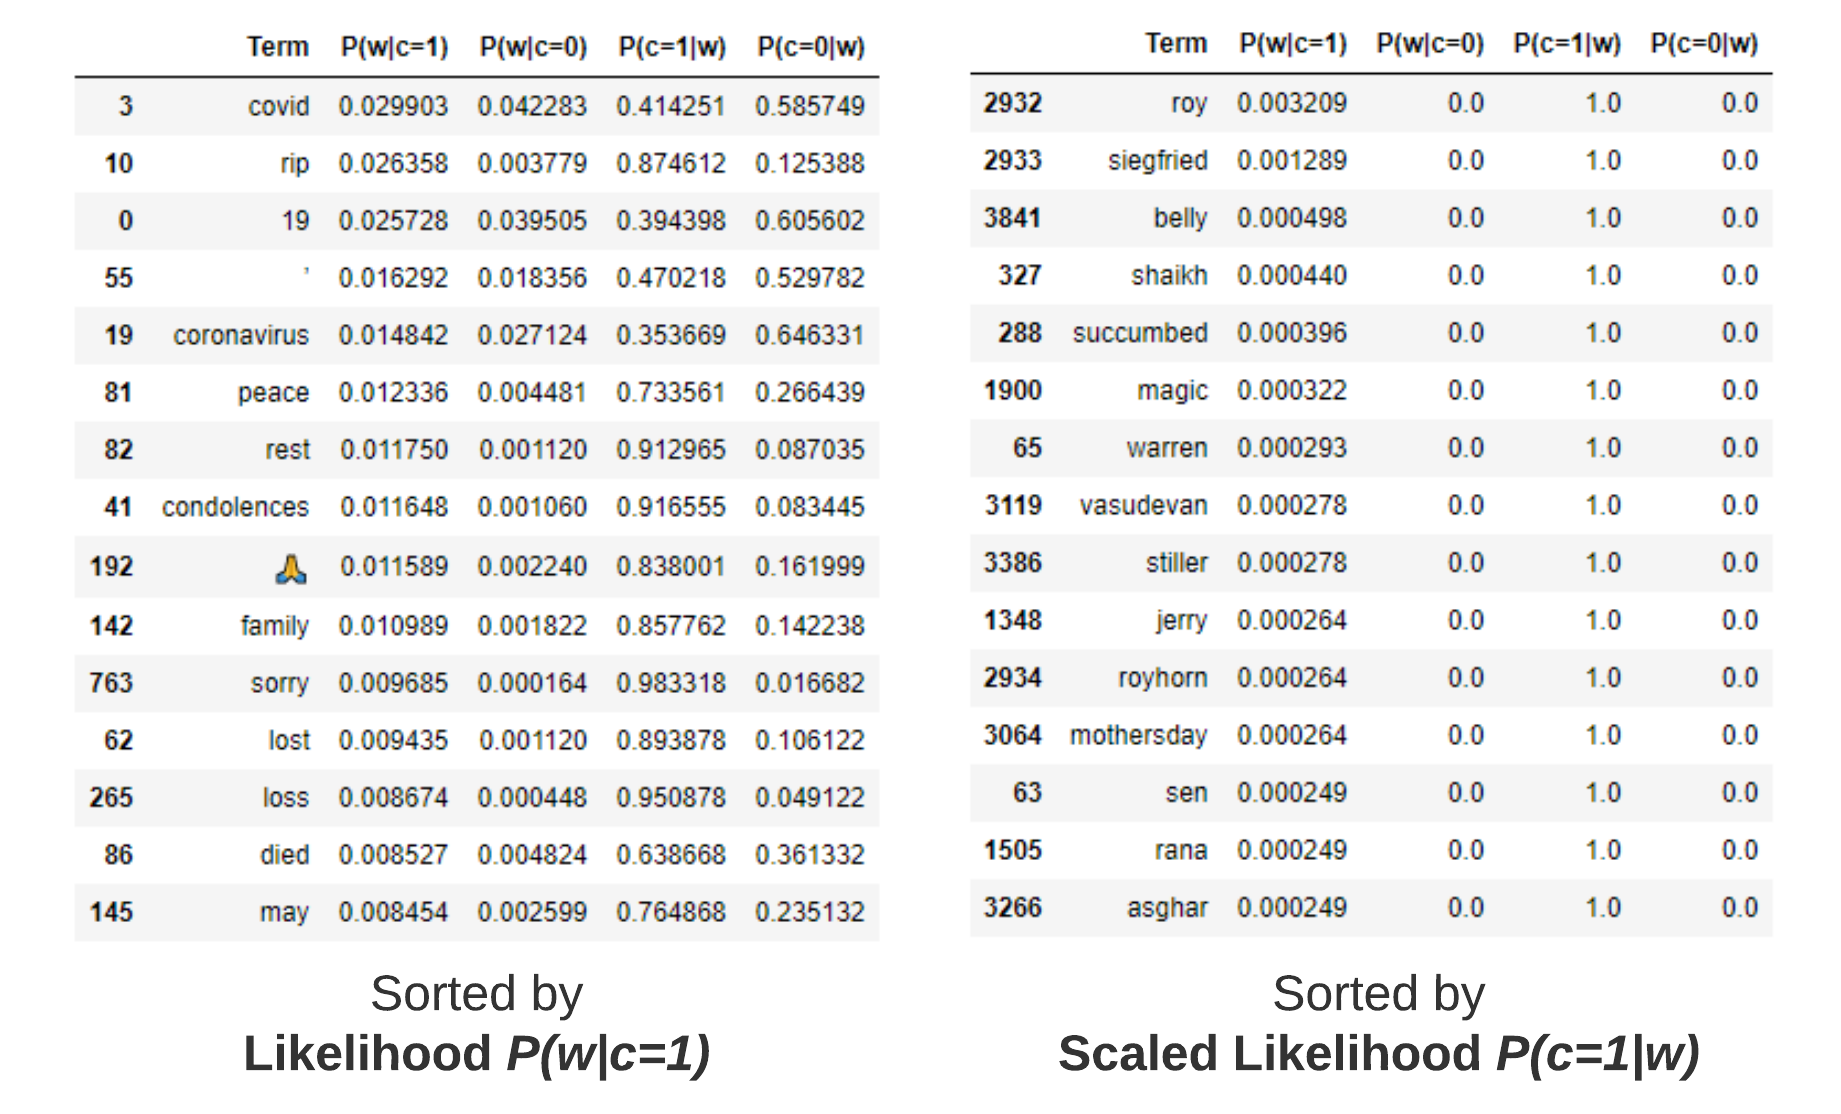
\includegraphics[width=\textwidth]{doc/images/EN_Lexicons.png}
\end{table}

\begin{table}[H]
    \caption{Resultado de los 15 emoticones con mayor probabilidad de aparecer en tweets de luto (\textit{mourning}) del \textit{dataset} en español (ES).}
    \label{tab:es_emojis}
    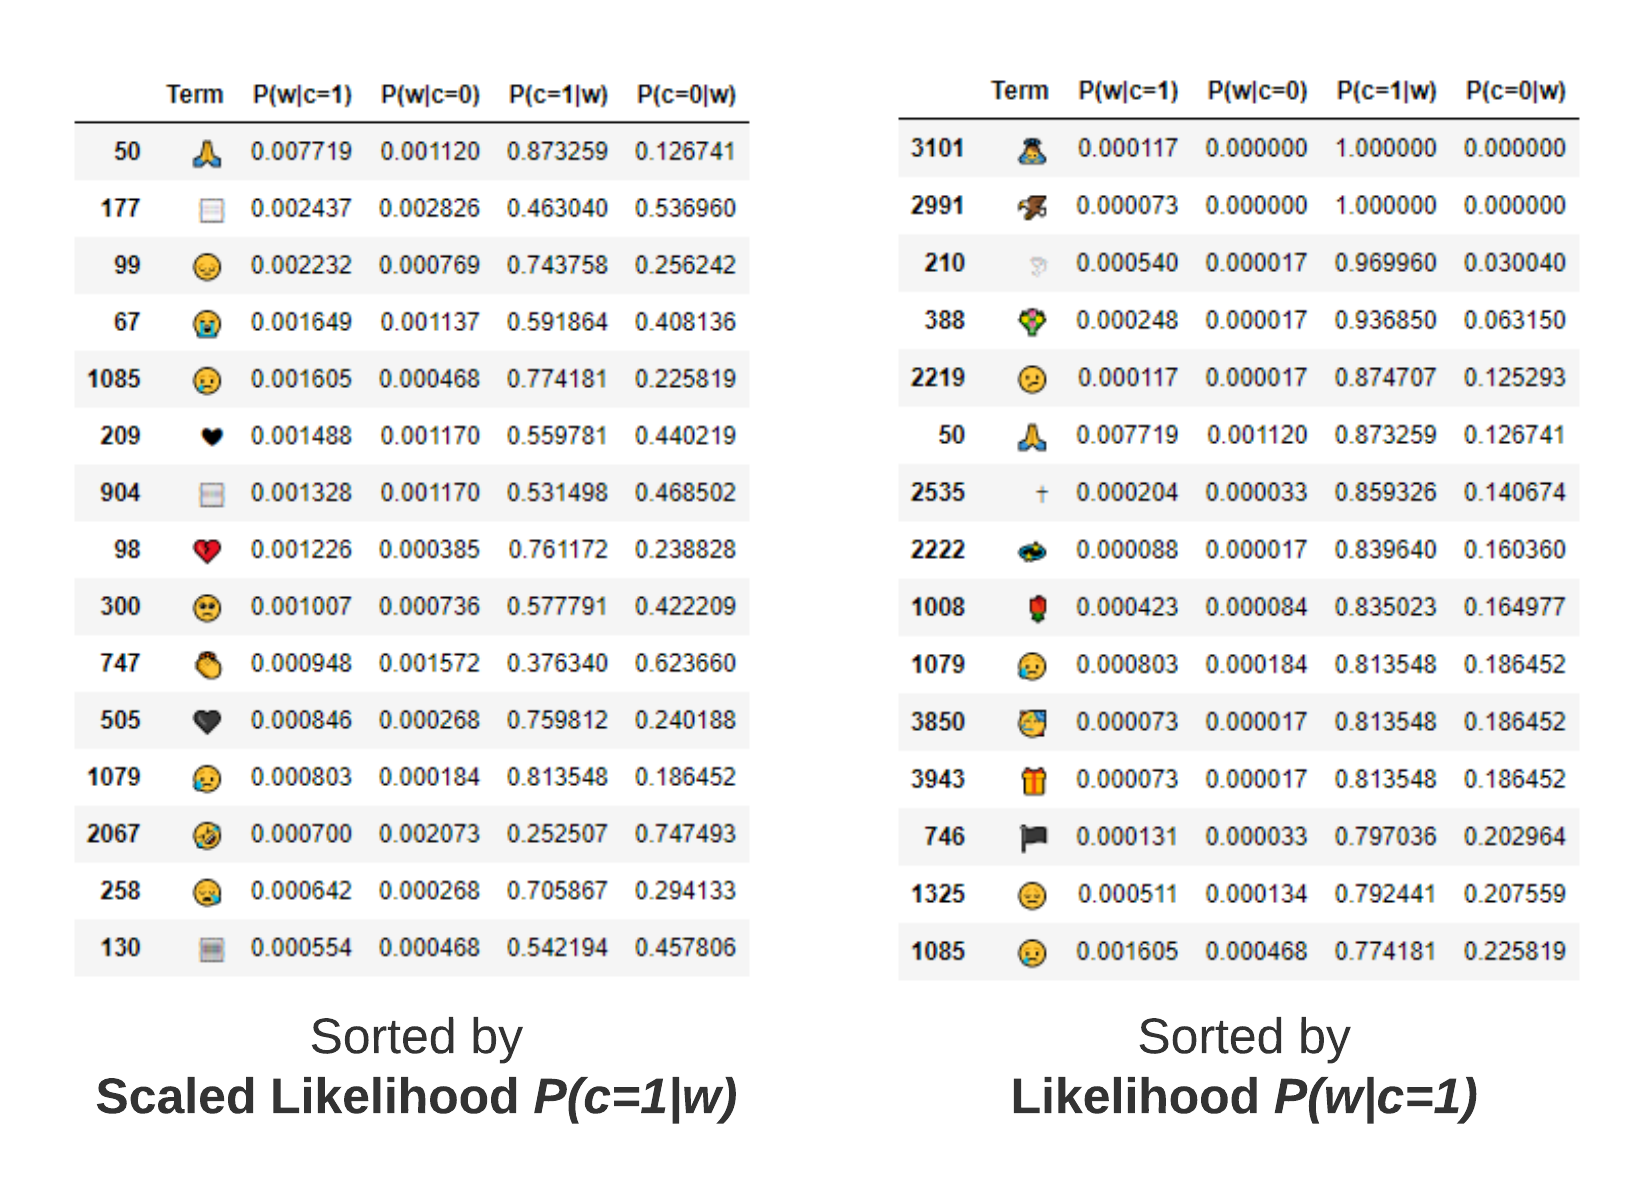
\includegraphics[width=\textwidth]{doc/images/ES_Emojis.png}
\end{table}

\begin{table}[H]
    \caption{Resultado de los 15 emoticones con mayor probabilidad de aparecer en tweets de luto (\textit{mourning}) del \textit{dataset} en español (ES).}
    \label{tab:en_emojis}
    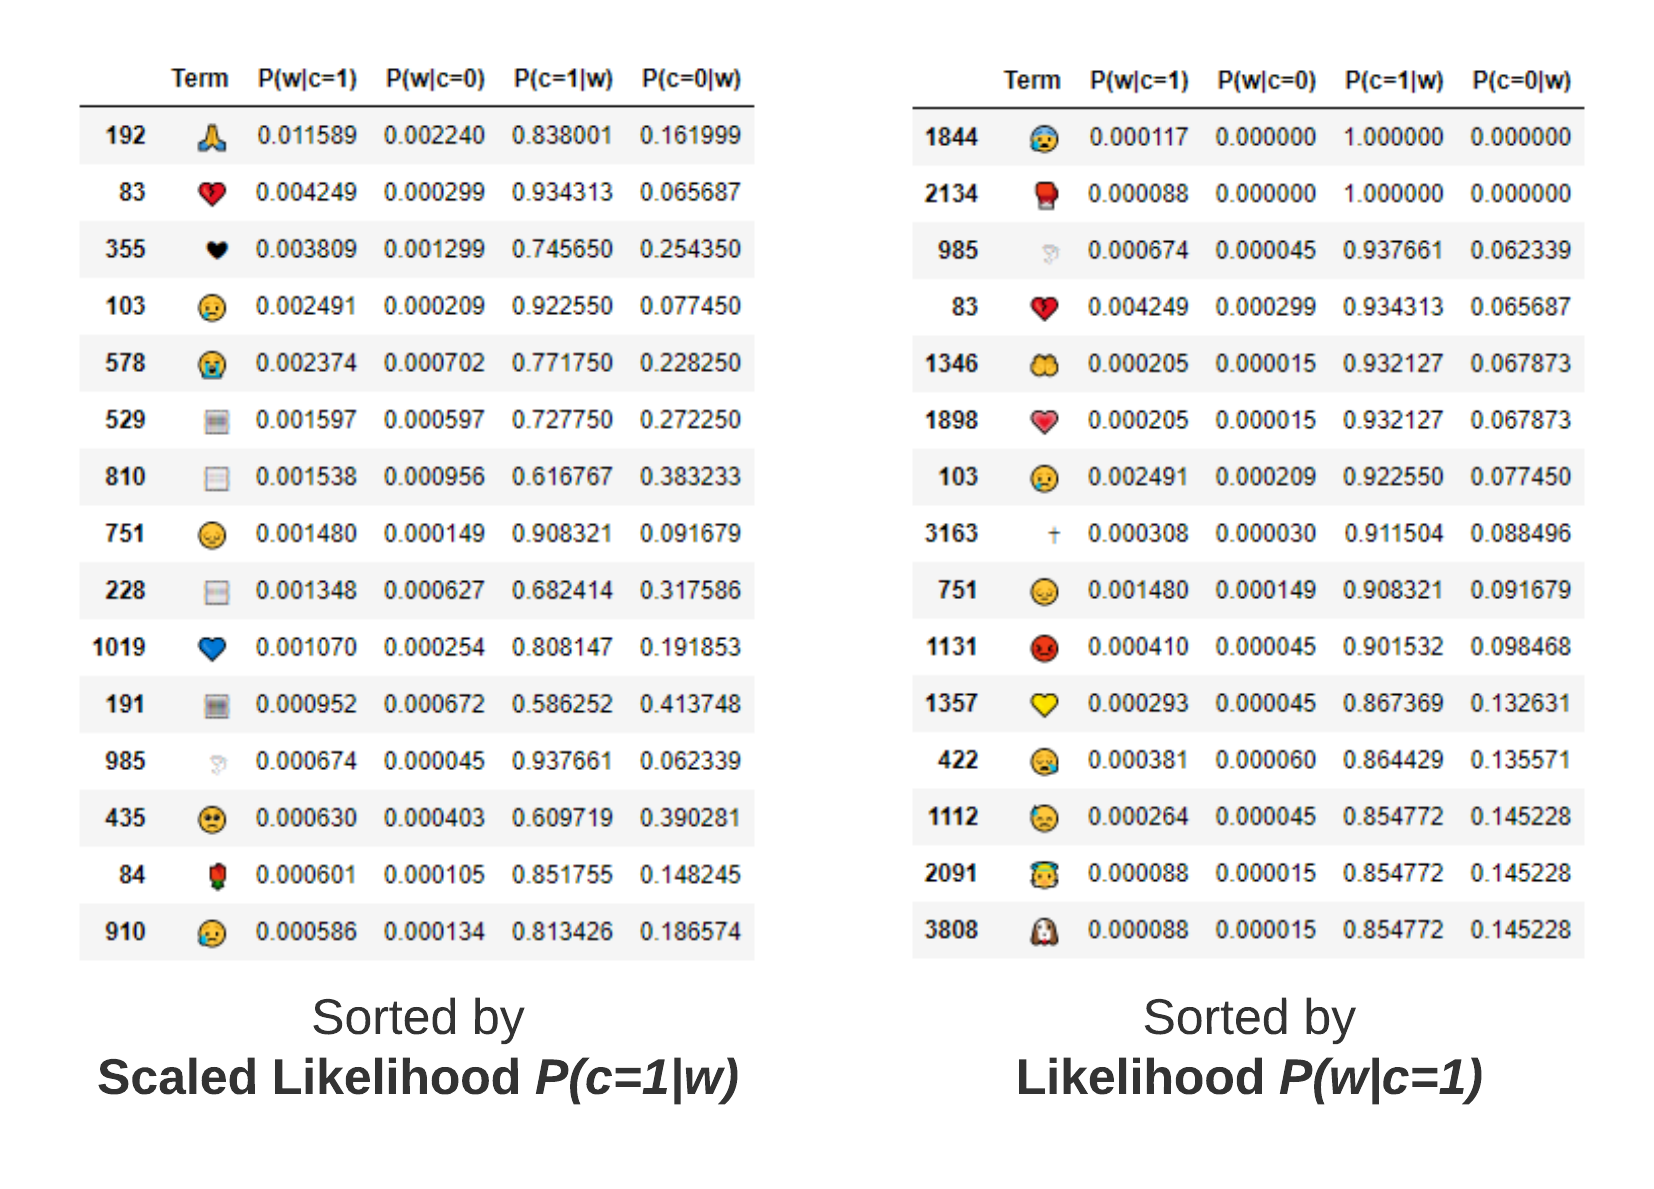
\includegraphics[width=\textwidth]{doc/images/EN_Emojis.png}
\end{table}

\subsection{Clasificadores}


\subsection{Análisis de importancia de características}